\documentclass{ximera}

\author{Anna Davis \and Rosemarie Emanuele} \title{Orthogonal Projections} \license{CC-BY 4.0}

\renewcommand{\vec}[1]{{\bf #1}}
\newcommand{\RR}{\mathbb{R}}
\newcommand{\dfn}{\textit}
\newcommand{\dotp}{\cdot}
\newcommand{\norm}[1]{\left\lVert#1\right\rVert}

\newtheorem{general}{Generalization}
\newtheorem{initprob}{Exploration Problem}
\usepackage{tikz-cd}
\usetikzlibrary{shapes.geometric}
\usetikzlibrary{arrows}
\pgfplotsset{compat=1.14}

\begin{document}
\begin{abstract}
 We find the projection of a vector onto a given non-zero vector, and find the distance between a point and a line.
\end{abstract}
\maketitle

\section*{Vector Projections}

Given a line $l$ and a vector $\vec{v}$ emanating from a point on $l$, it is sometimes convenient to express $\vec{v}$ as the sum of a vector $\vec{v}_{\parallel}$, parallel to $l$, and a vector $\vec{v}_{\perp}$, perpendicular to $l$.

\begin{image}[2in]
 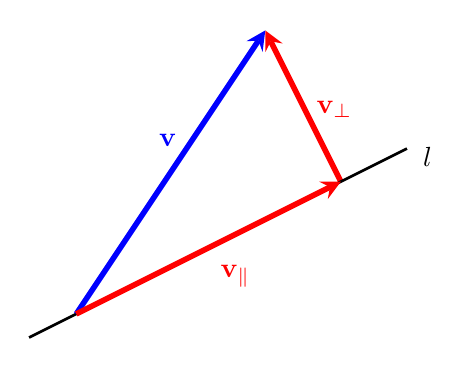
\begin{tikzpicture}[scale=.6]
  \draw[line width=2pt,red,-stealth](3.6, 0.8)--(2,4) node[below=10mm, right=5mm]{$\vec{v}_{\perp}$};
   \draw [-,line width=1pt]  (-3,-2.5)--(5, 1.5)node[below=1mm, right=2]{$l$};
\draw[line width=2pt,blue,-stealth](-2, -2)node[above=22mm, right=9mm]{$\vec{v}$}--(2,4);
\draw[line width=2pt,red,-stealth](-2, -2)--(3.6, 0.8) node[below=12mm, left=10mm]{$\vec{v}_{\parallel}$};
\end{tikzpicture}

\end{image}

Suppose $\vec{d}$ is a direction vector for $l$.  Then $\vec{v}_
{\parallel}=k\vec{d}$ for some scalar $k$.  Our goal is to find $k$.  
\begin{align*}\vec{v}\dotp\vec{d}&=(\vec{v}_{\parallel}+\vec{v}_{\perp})\dotp\vec{d}\\
&=(k\vec{d}+\vec{v}_{\perp})\dotp\vec{d}\\
&=k\vec{d}\dotp\vec{d}+\vec{v}_{\perp}\dotp\vec{d}\\
&=k\norm{\vec{d}}^2+0\\
&=k\norm{\vec{d}}^2
\end{align*}
We conclude that $$k=\frac{\vec{v}\dotp\vec{d}}{\norm{\vec{d}}^2}$$
and $$\vec{v}_{\parallel}=k\vec{d}=\left(\frac{\vec{v}\dotp\vec{d}}{\norm{\vec{d}}^2}\right)\vec{d}$$

The vector $\vec{v}_{\parallel}=\left(\frac{\vec{v}\dotp\vec{d}}{\norm{\vec{d}}^2}\right)\vec{d}$ is called the \dfn{projection of $\vec{v}$ onto $\vec{d}$}.  In our discussion, $\vec{d}$ is a direction vector for line $l$.  So, we can also say that $\vec{v}_{\parallel}$ is the \dfn{projection of $\vec{v}$ onto $l$}.

To find $\vec{v}_{\perp}$, observe that $\vec{v}_{\perp}=\vec{v}-\vec{v}_{\parallel}$.


\begin{definition}\label{def:projection}
Let $\vec{v}$ be a vector, and let $\vec{d}$ be a non-zero vector.  The projection of $\vec{v}$ onto $\vec{d}$ is given by 
$$\text{proj}_{\vec{d}}\vec{v}=\left(\frac{\vec{v}\dotp\vec{d}}{\norm{\vec{d}}^2}\right)\vec{d}$$
\end{definition}

\begin{example}
Find the projection of $\vec{v}$, shown below, onto the line given by $y=\frac{1}{2}x-1$.

\begin{image}[2.5in]
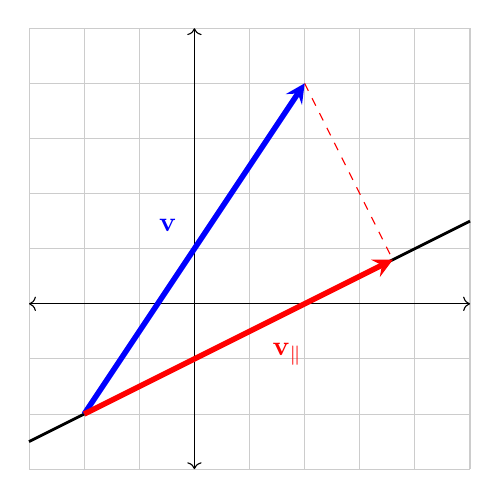
\begin{tikzpicture}[scale=.7]

\draw[thin,gray!40] (-3,-3) grid (5,5);
  \draw[<->] (-3,0)--(5,0);
  \draw[<->] (0,-3)--(0,5);
  \draw[red, dashed] (2,4)--(3.6, 0.8); 
  \draw [-,line width=1pt]  (-3,-2.5)--(5, 1.5);
\draw[line width=2pt,blue,-stealth](-2, -2)node[above=24mm, right=8mm]{$\vec{v}$}--(2,4);
\draw[line width=2pt,red,-stealth](-2, -2)--(3.6, 0.8) node[below=12mm, left=10mm]{$\vec{v}_{\parallel}$};
\end{tikzpicture}
\end{image}

\begin{explanation}
We begin by finding vectors $\vec{v}$ and $\vec{d}$. The tail of $\vec{v}$ is located at $(-2, -2)$, and the head of $\vec{v}$ is at $(2, 4)$.  Using the ``head-tail" formula we get 
$$\vec{v}=\begin{bmatrix}2-(-2)\\4-(-2)\end{bmatrix}=\begin{bmatrix}4\\6\end{bmatrix}$$ The direction vector for the line $y=\frac{1}{2}x-1$ is $$\vec{d}=\begin{bmatrix}2\\1\end{bmatrix}$$
We find that $\vec{v}\dotp\vec{d}=14$ and $\norm{\vec{d}}^2=5$.
Thus $$\text{proj}_{\vec{d}}\vec{v}=\left(\frac{\vec{v}\dotp\vec{d}}{\norm{\vec{d}}^2}\right)\vec{d}=\frac{14}{5}\begin{bmatrix}2\\1\end{bmatrix}=\begin{bmatrix}28/5\\14/5\end{bmatrix}$$
\end{explanation}
\end{example}

\section*{Distance from a Point to a Line}

The shortest distance from a point to a line is the length of the perpendicular line segment dropped from the point to the line.  Vector projection formula will help us find the length of such a perpendicular.

\begin{example}
Let $A(2, -1, 1)$ be a point in $\RR^3$.  Suppose line $l$ is given by parametric equations $$x=t+3$$
$$y=-t+1$$
$$z=t-2$$

\begin{image}[2in]
\begin{tikzpicture}[scale=.6]
  
   \draw [-,line width=1pt]  (-3,-2.5)--(5, 1.5)node[below=1mm, right=2]{$l$};
   
\fill (2, 4)node[above=2mm, right=1mm]{$A(2, -1, 1)$} circle (1mm);
\end{tikzpicture}
\end{image}

Find the distance from $A$ to $l$.
\begin{explanation}
We will first construct a vector $\vec{v}$ by picking an arbitrary point $B$ on $l$ to be the tail of $\vec{v}$ and using point $A$ as the head of $\vec{v}$.  An easy point to choose on line $l$ is the point $(3, 1, -2)$ that corresponds to $t=0$.  Now we have 
$$\vec{v}=\overrightarrow{BA}=\begin{bmatrix}2-3\\-1-1\\1-(-2)\end{bmatrix}=\begin{bmatrix}-1\\-2\\3\end{bmatrix}$$

\begin{image}[2in]
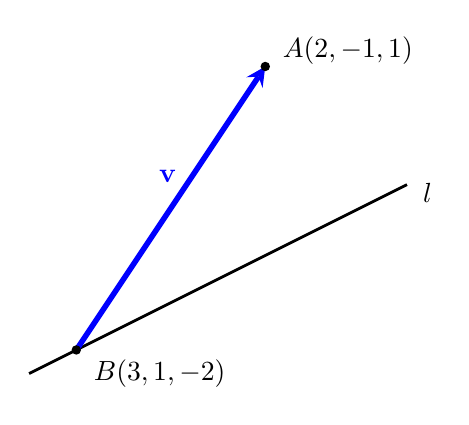
\begin{tikzpicture}[scale=.6]
  
   \draw [-,line width=1pt]  (-3,-2.5)--(5, 1.5)node[below=1mm, right=2]{$l$};
   
\draw[line width=2pt,blue,-stealth](-2, -2)node[above=22mm, right=9mm]{$\vec{v}$}--(2,4);

\fill (-2, -2) node[below=3mm, right=1mm]{$B(3, 1, -2)$} circle (1mm);
\fill (2, 4)node[above=2mm, right=1mm]{$A(2, -1, 1)$} circle (1mm);
\end{tikzpicture}
\end{image}

The line has a direction vector 
$$\vec{d}=\begin{bmatrix}1\\-1\\1\end{bmatrix}$$

We will now find the projection of $\overrightarrow{BA}$ onto $l$  $$\text{proj}_{\vec{d}} \overrightarrow{BA}=\left(\frac{\vec{v}\dotp\vec{d}}{\norm{\vec{d}}^2}\right)\vec{d}=\frac{4}{3}\begin{bmatrix}1\\-1\\1\end{bmatrix}=\begin{bmatrix}4/3\\-4/3\\4/3\end{bmatrix}$$

\begin{image}[2in]
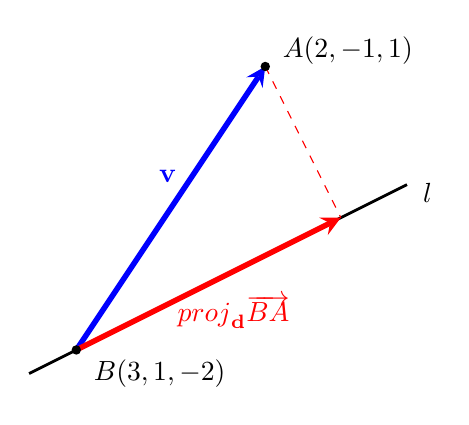
\begin{tikzpicture}[scale=.6]
  
   \draw [-,line width=1pt]  (-3,-2.5)--(5, 1.5)node[below=1mm, right=2]{$l$};
   
\draw[line width=2pt,blue,-stealth](-2, -2)node[above=22mm, right=9mm]{$\vec{v}$}--(2,4);
\draw[line width=2pt,red,-stealth](-2, -2)--(3.6, 0.8) node[below=12mm, left=5mm]{$\text{proj}_{\vec{d}}\overrightarrow{BA}$};
\draw[red, dashed] (2,4)--(3.6, 0.8); 
\fill (-2, -2) node[below=3mm, right=1mm]{$B(3, 1, -2)$} circle (1mm);
\fill (2, 4)node[above=2mm, right=1mm]{$A(2, -1, 1)$} circle (1mm);
\end{tikzpicture}
\end{image}


Next, we find $\vec{v}_{\perp}$.
$$\vec{v}_{\perp}=\vec{v}-\vec{v}_{\parallel}=\begin{bmatrix}-1\\-2\\3\end{bmatrix}-\begin{bmatrix}4/3\\-4/3\\4/3\end{bmatrix}=\begin{bmatrix}-7/3\\-2/3\\5/3\end{bmatrix}$$

\begin{image}[2in]
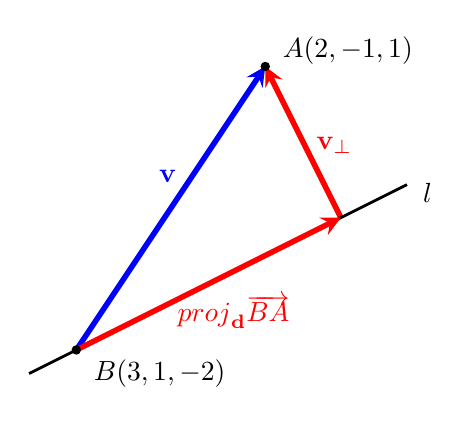
\begin{tikzpicture}[scale=.6]
  \draw[line width=2pt,red,-stealth](3.6, 0.8)--(2,4) node[below=10mm, right=5mm]{$\vec{v}_{\perp}$};
   \draw [-,line width=1pt]  (-3,-2.5)--(5, 1.5)node[below=1mm, right=2]{$l$};
   
\draw[line width=2pt,blue,-stealth](-2, -2)node[above=22mm, right=9mm]{$\vec{v}$}--(2,4);
\draw[line width=2pt,red,-stealth](-2, -2)--(3.6, 0.8) node[below=12mm, left=5mm]{$\text{proj}_{\vec{d}}\overrightarrow{BA}$};
\fill (-2, -2) node[below=3mm, right=1mm]{$B(3, 1, -2)$} circle (1mm);
\fill (2, 4)node[above=2mm, right=1mm]{$A(2, -1, 1)$} circle (1mm);
\end{tikzpicture}
\end{image}


Finally, to find the distance between point $A$ and line $l$, we find the magnitude of $\vec{v}_{\perp}$.
$$\norm{\vec{v}_{\perp}}=\frac{1}{3}\sqrt{49+4+25}=\frac{\sqrt{78}}{3}$$
\end{explanation}
\end{example}

\section*{Practice Problems}
\begin{problem}
Find $\text{proj}_{\vec{d}}\vec{v}$.  Enter your answers in decimal form.
  \begin{problem}
  If $\vec{d}=\begin{bmatrix}-1\\3\end{bmatrix}$ and $\vec{v}=\begin{bmatrix}1\\4\end{bmatrix}$ then
  $$\text{proj}_{\vec{d}}\vec{v}=\begin{bmatrix}\answer{-1.1}\\\answer{3.3}\end{bmatrix}$$
    \end{problem}
    \begin{problem}
    If $\vec{d}=\begin{bmatrix}0\\2\\1\end{bmatrix}$ and $\vec{v}=\begin{bmatrix}-1\\-4\\2\end{bmatrix}$ then
    $$\text{proj}_{\vec{d}}\vec{v}=\begin{bmatrix}\answer{0}\\\answer{-2.4}\\\answer{-1.2}\end{bmatrix}$$
    \end{problem}
\end{problem}
\begin{problem}
Find the projection of vector $\vec{v}$ onto line $l$.

\begin{image}
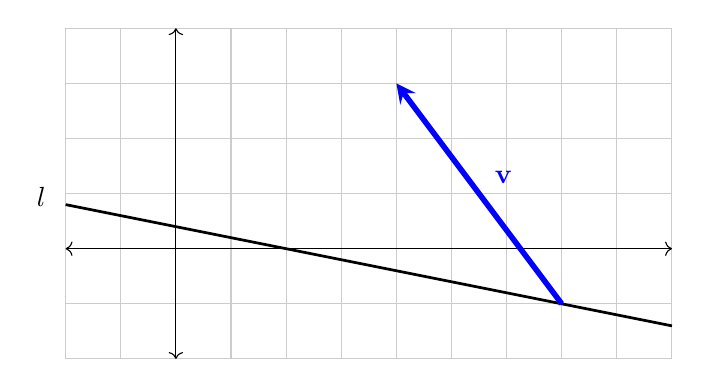
\begin{tikzpicture}[scale=.7]
\draw[thin,gray!40] (-2,-2) grid (9,4);
  \draw[<->] (-2,0)--(9,0);
  \draw[<->] (0,-2)--(0,4);
  
  \draw [-,line width=1pt]  (-2,0.8)node[above=1mm, right=-5mm]{$l$}--(9, -1.4);
\draw[line width=2pt,blue,-stealth](7, -1)node[above=16mm, right=-10mm]{$\vec{v}$}--(4,3);
\end{tikzpicture}
\end{image}

Answer:
$$\begin{bmatrix}\answer{-95/26}\\\answer{19/26}\end{bmatrix}$$
\end{problem}
\begin{problem}
Find the distance between point $A$ and line $l$.

\begin{image}
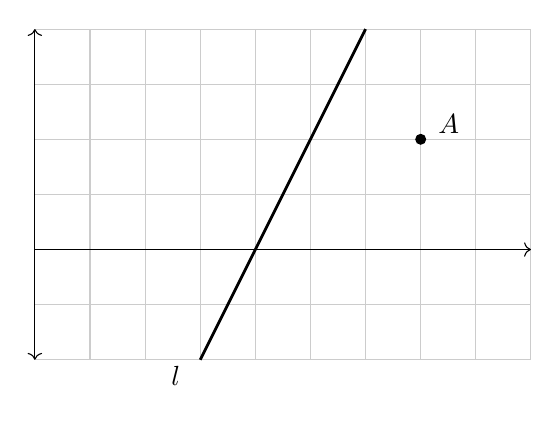
\begin{tikzpicture}[scale=.7]
\draw[thin,gray!40] (0,-2) grid (9,4);
  \draw[->] (0,0)--(9,0);
  \draw[<->] (0,-2)--(0,4);
  \fill (7,2)node[above=2mm, right=1mm]{$A$} circle (1mm);
  \draw [-,line width=1pt]  (3,-2)node[below=2mm, right=-5mm]{$l$}--(6, 4);
\end{tikzpicture}
\end{image}

Answer: $\sqrt{\answer{3.2}}$.
\end{problem}
\begin{problem}
Show that $\text{proj}_{\vec{d}}\vec{v}$ does not depend on the length of $\vec{d}$ by proving that $\text{proj}_{\vec{d}}\vec{v}=\text{proj}_{k\vec{d}}\vec{v}$ for $k\neq 0$.  What does this result mean geometrically?  Illustrate your response with a diagram.
\end{problem}
\begin{problem}
Find the equation of a circle centered at $(4, 2)$ if the line $y=\frac{3}{2}x+3$ is tangent to the circle.

The equation of the circle is:
$$(x-4)^2+(y-2)^2=\answer{196/13}$$
\end{problem}
\end{document}
